\section{Modellazione CAD 3D}
Di seguito si riportano i modelli CAD 3D del riduttore realizzati con il software SOLIDWORKS.\\
\\
\begin{figure}[h]
\centering
   {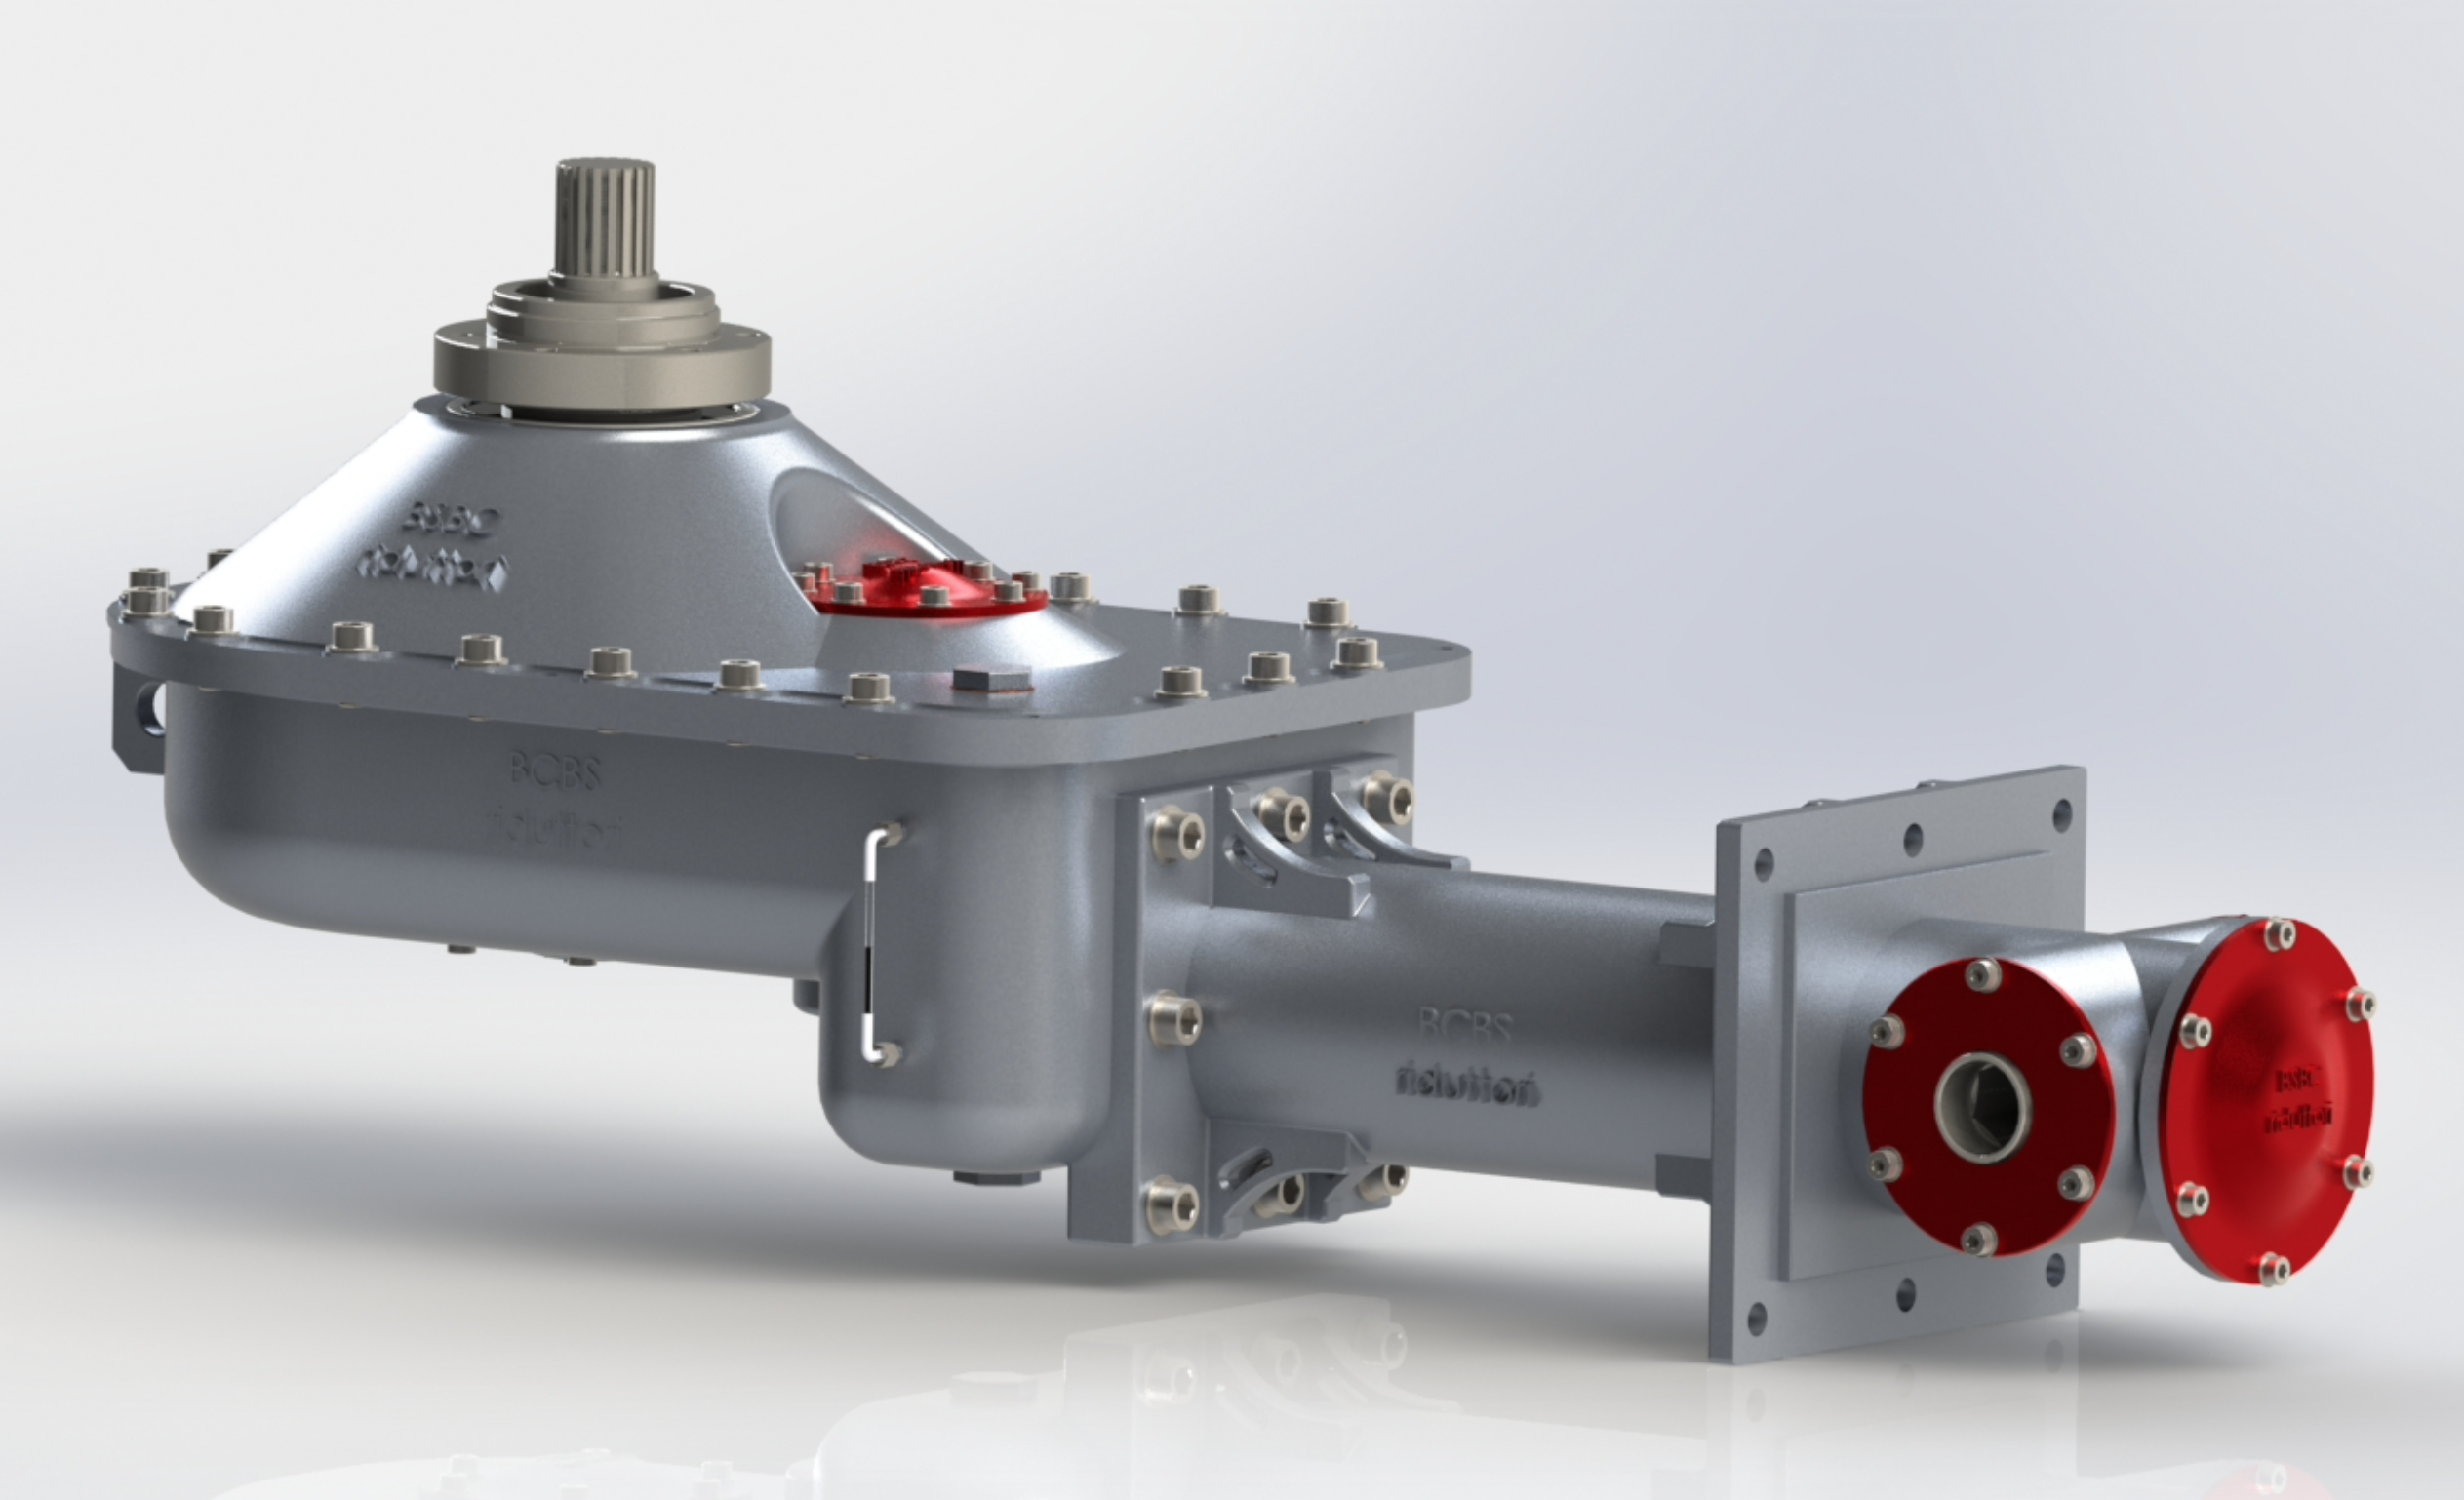
\includegraphics[scale=0.3]{Immagini/RenderingRiduttore2.png}} 
   {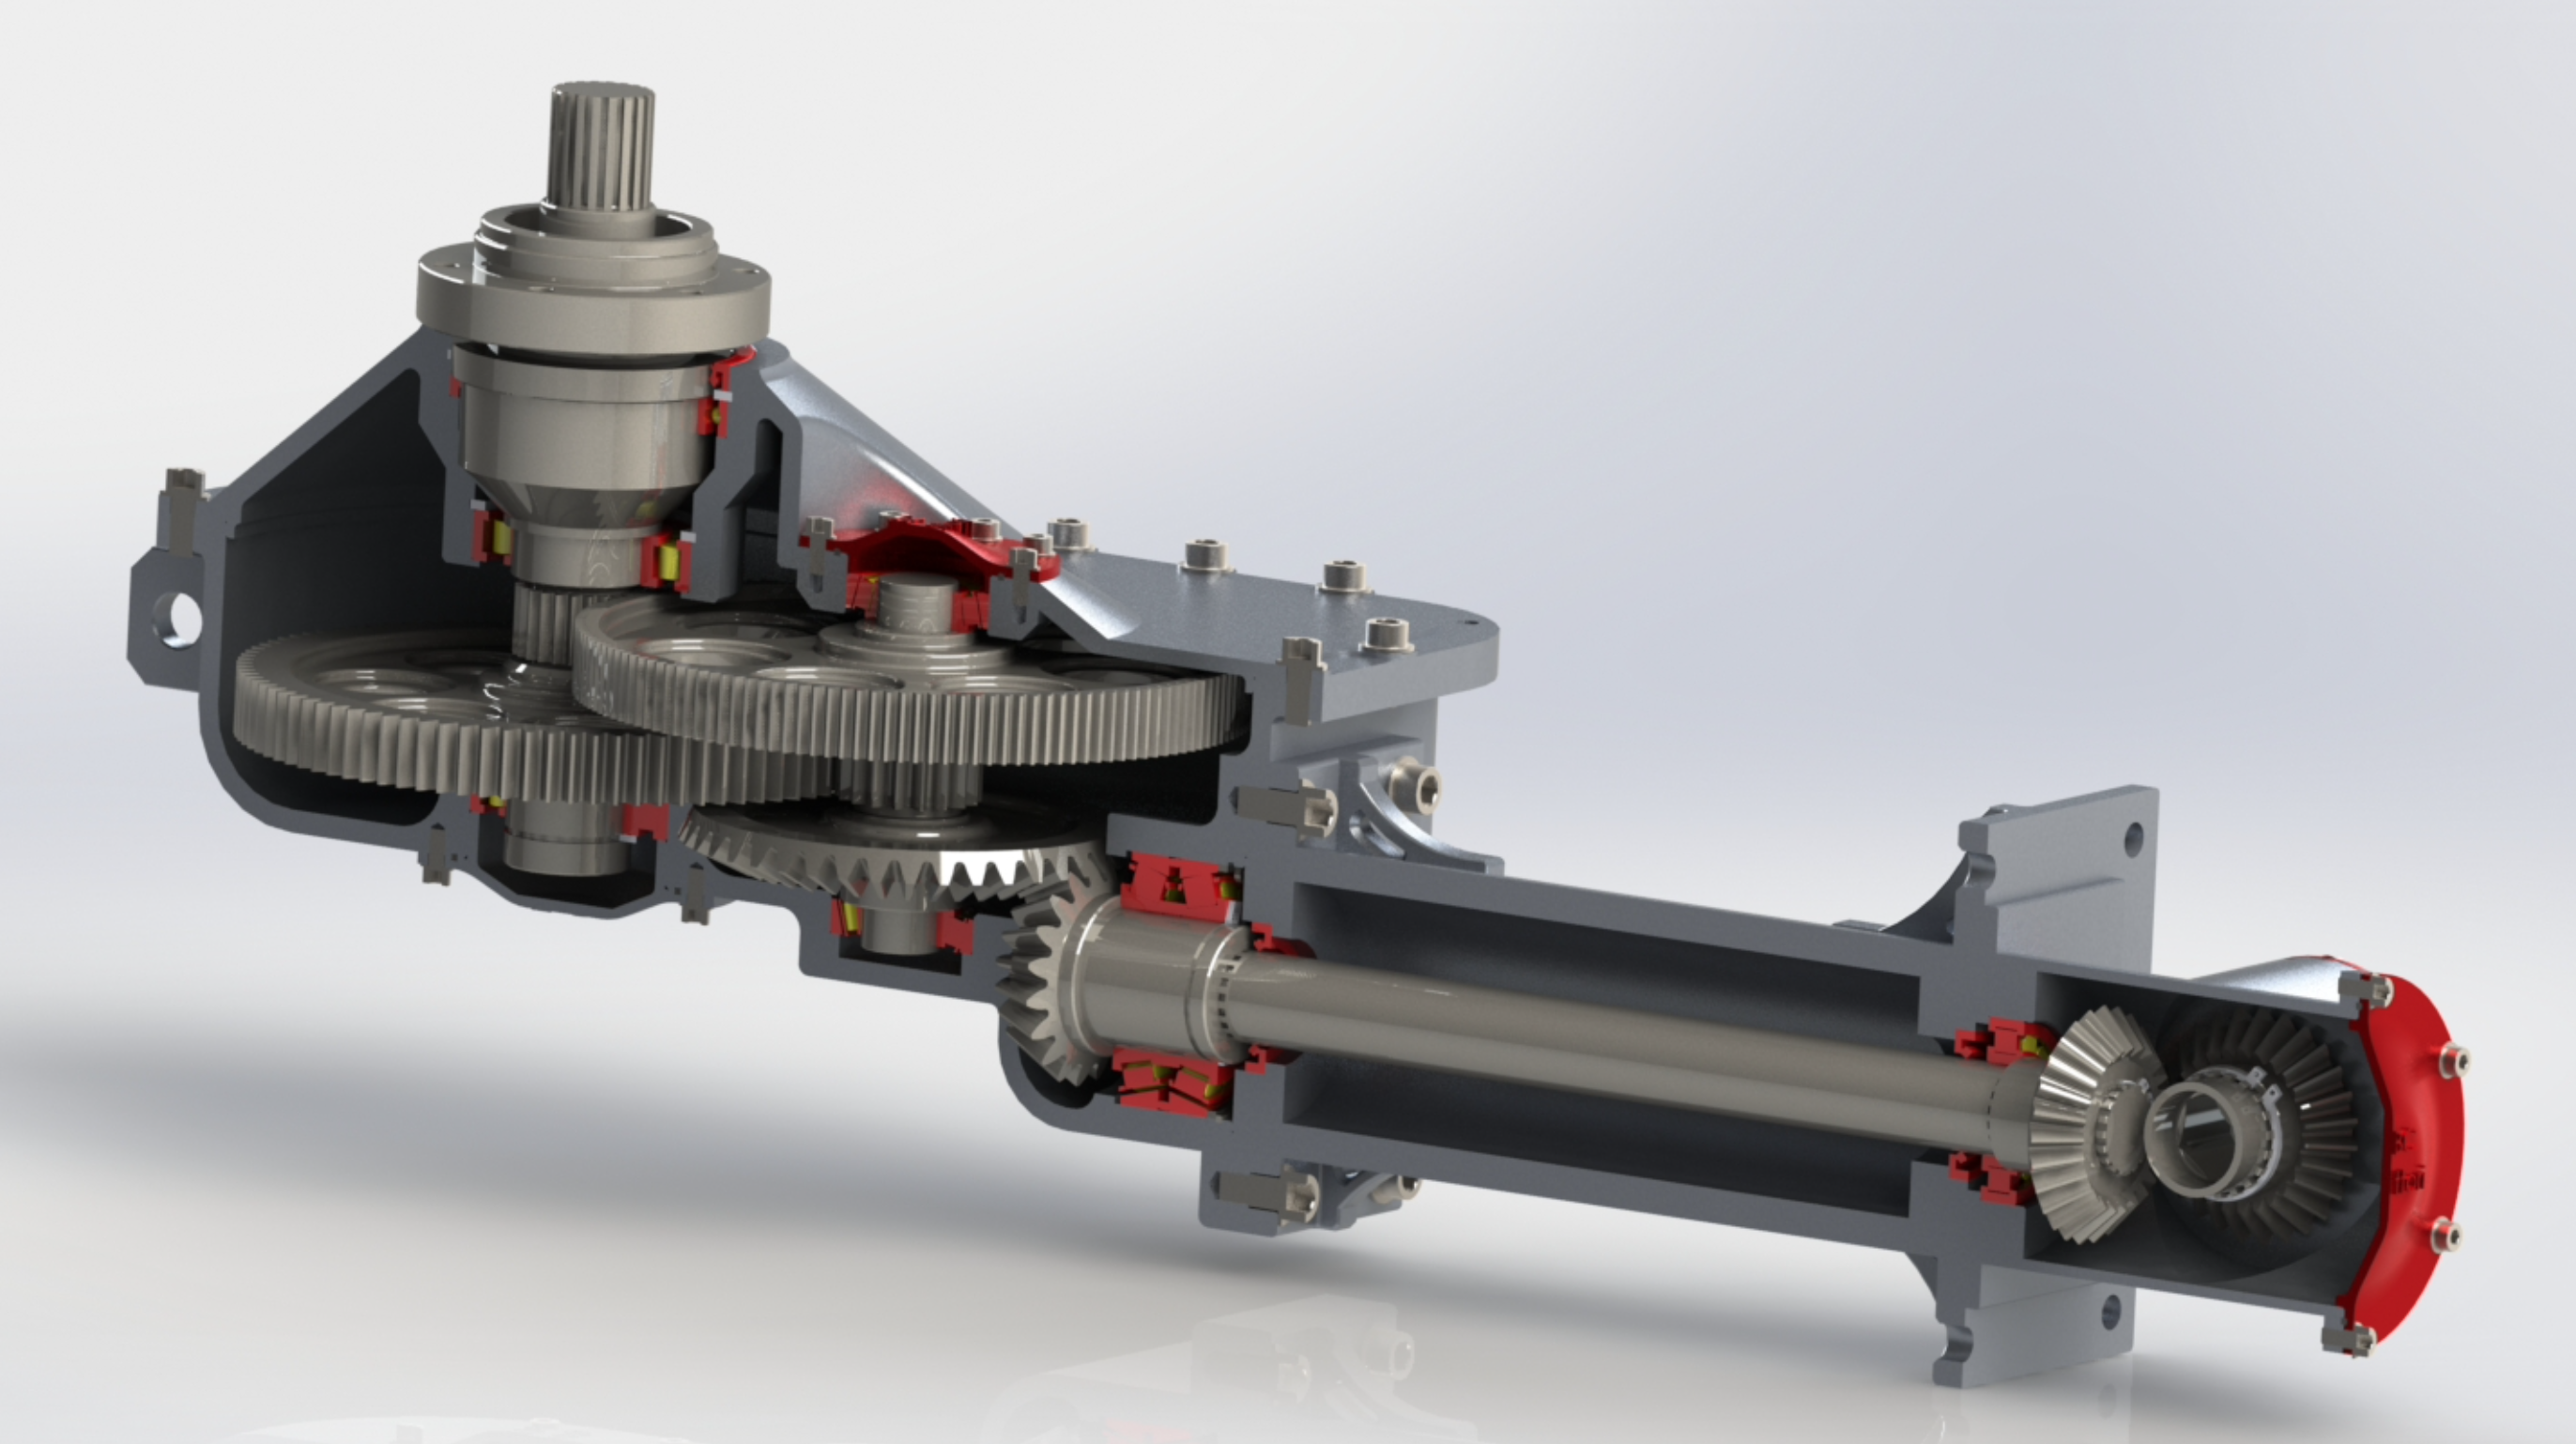
\includegraphics[scale=0.275]{Immagini/RenderingRiduttore1.png}} 
\caption{Rendering riduttore modellato tramite software SOLIDWORKS}
\label{fig:riduttore12}
\end{figure}
\newpage
\begin{figure}[h]
    \centering
     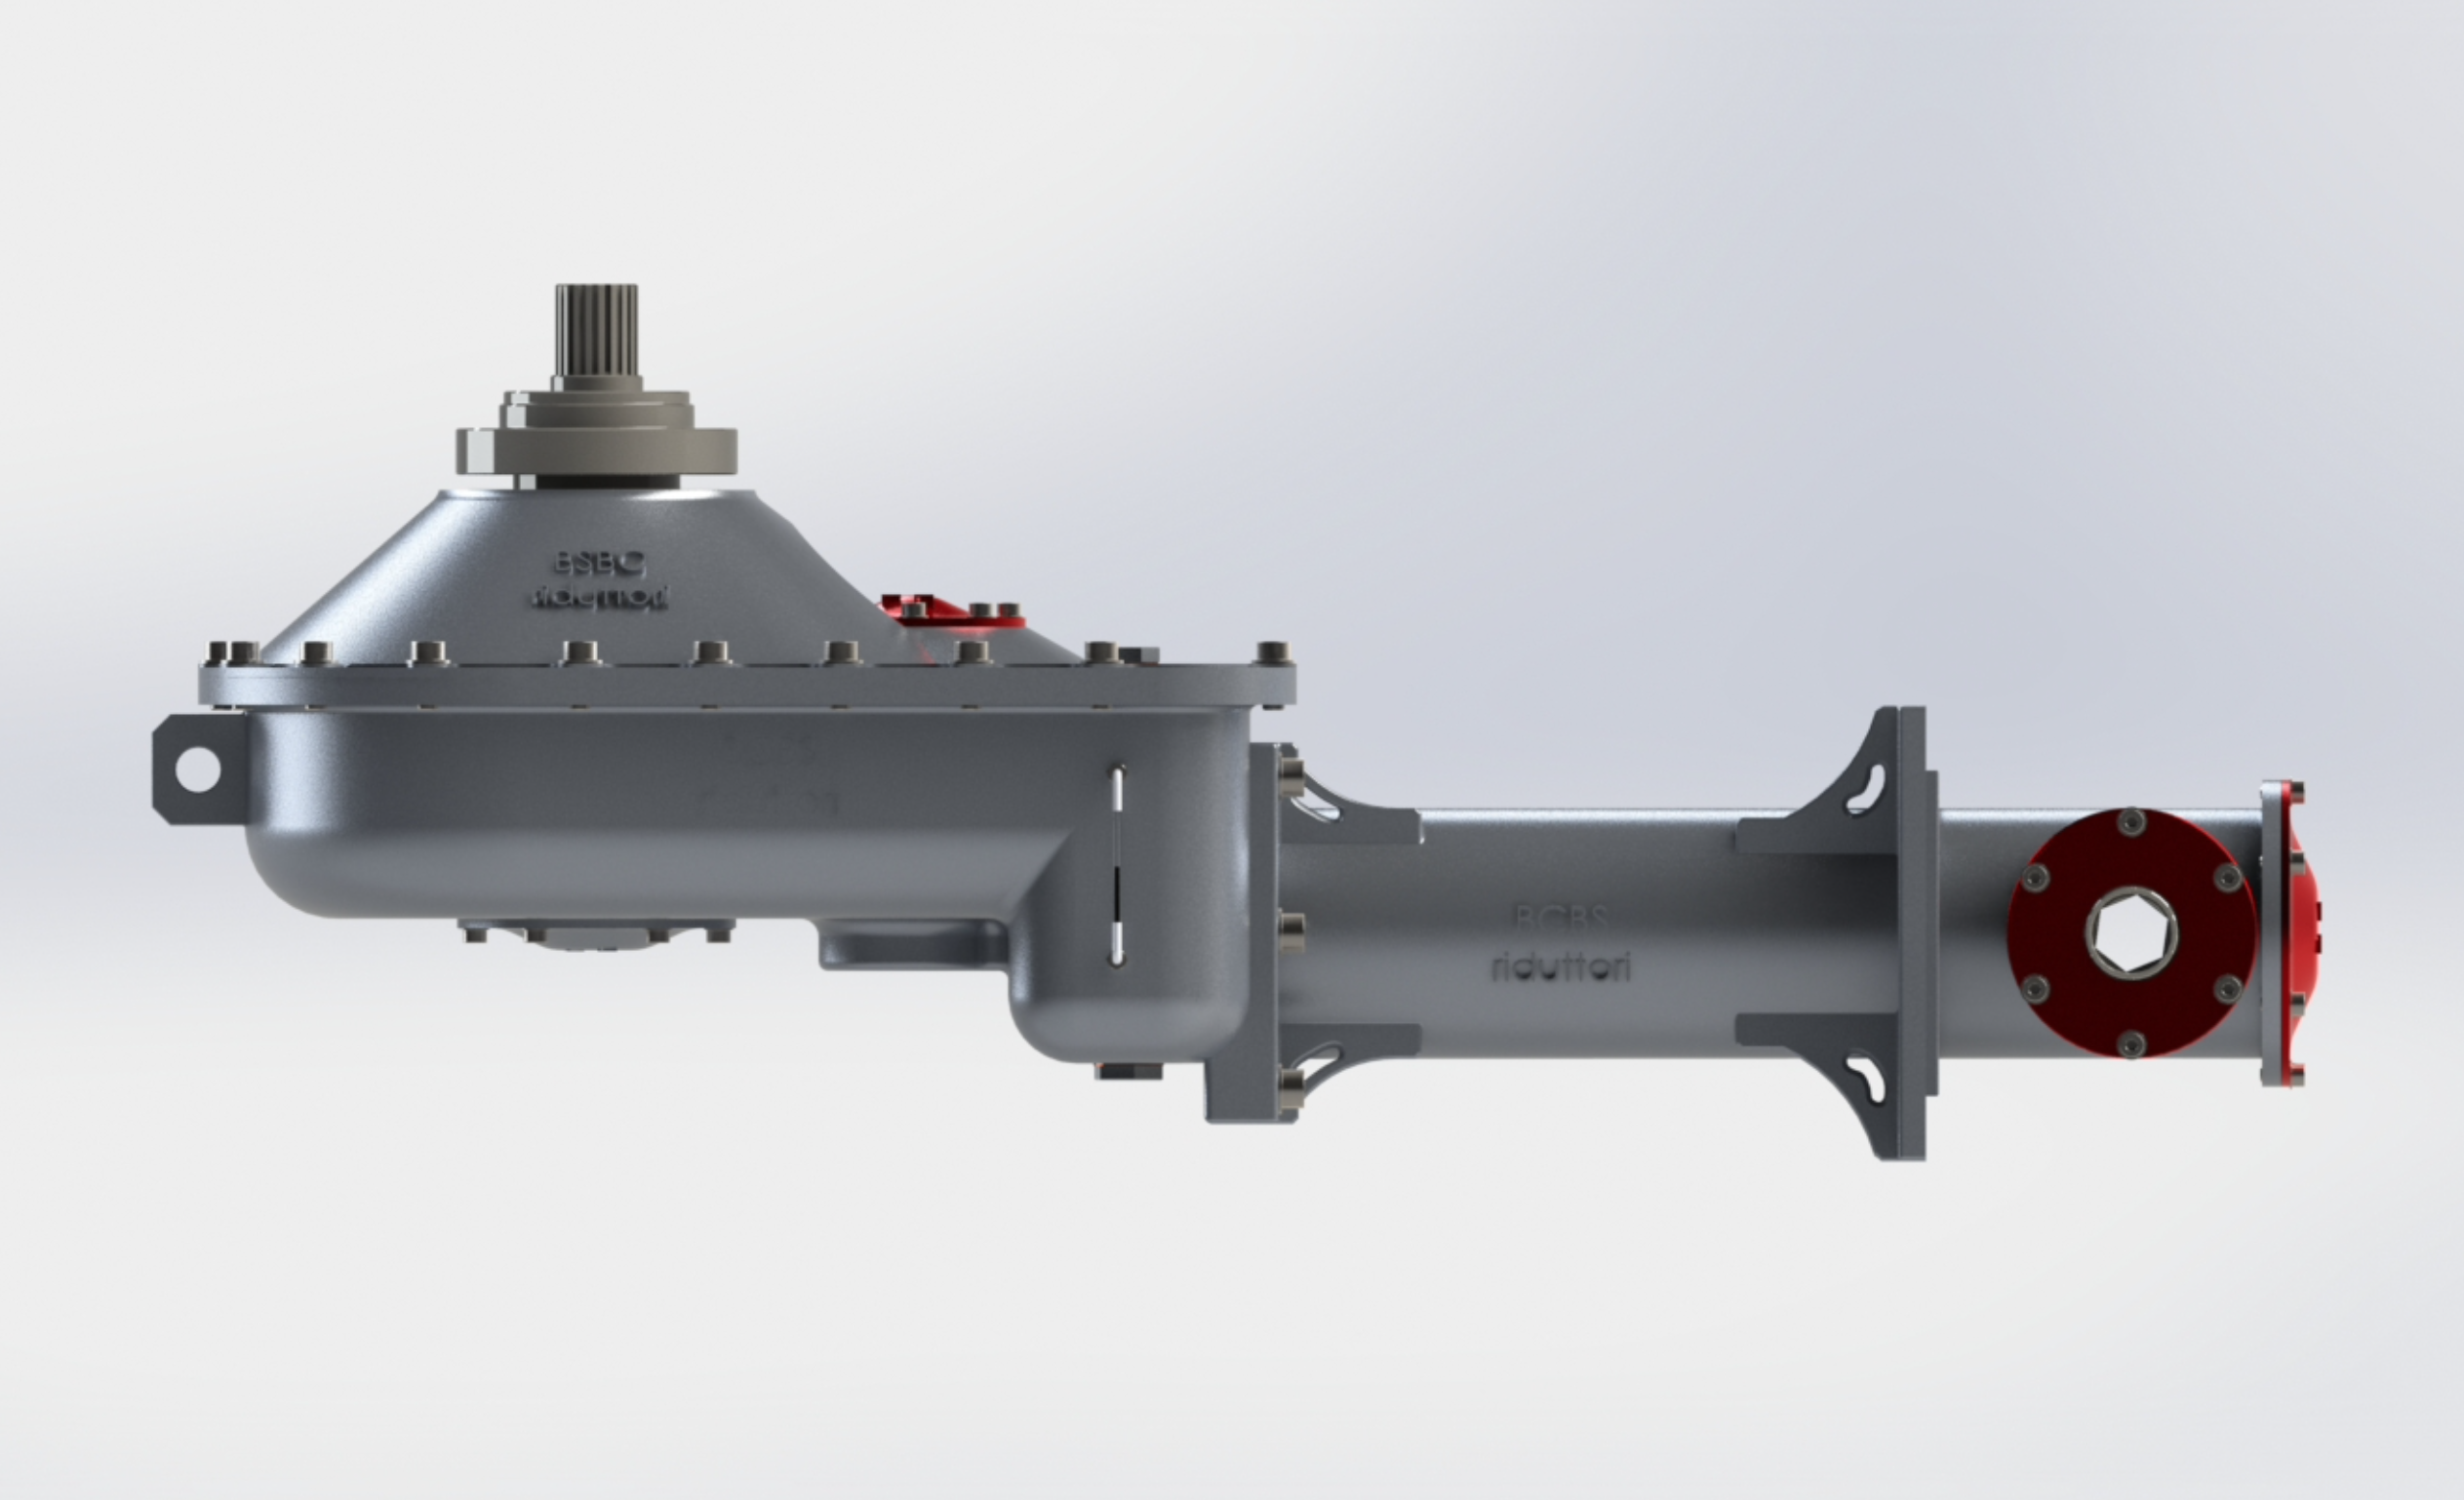
\includegraphics[scale=0.3]{Immagini/RenderingRiduttore3.png}
    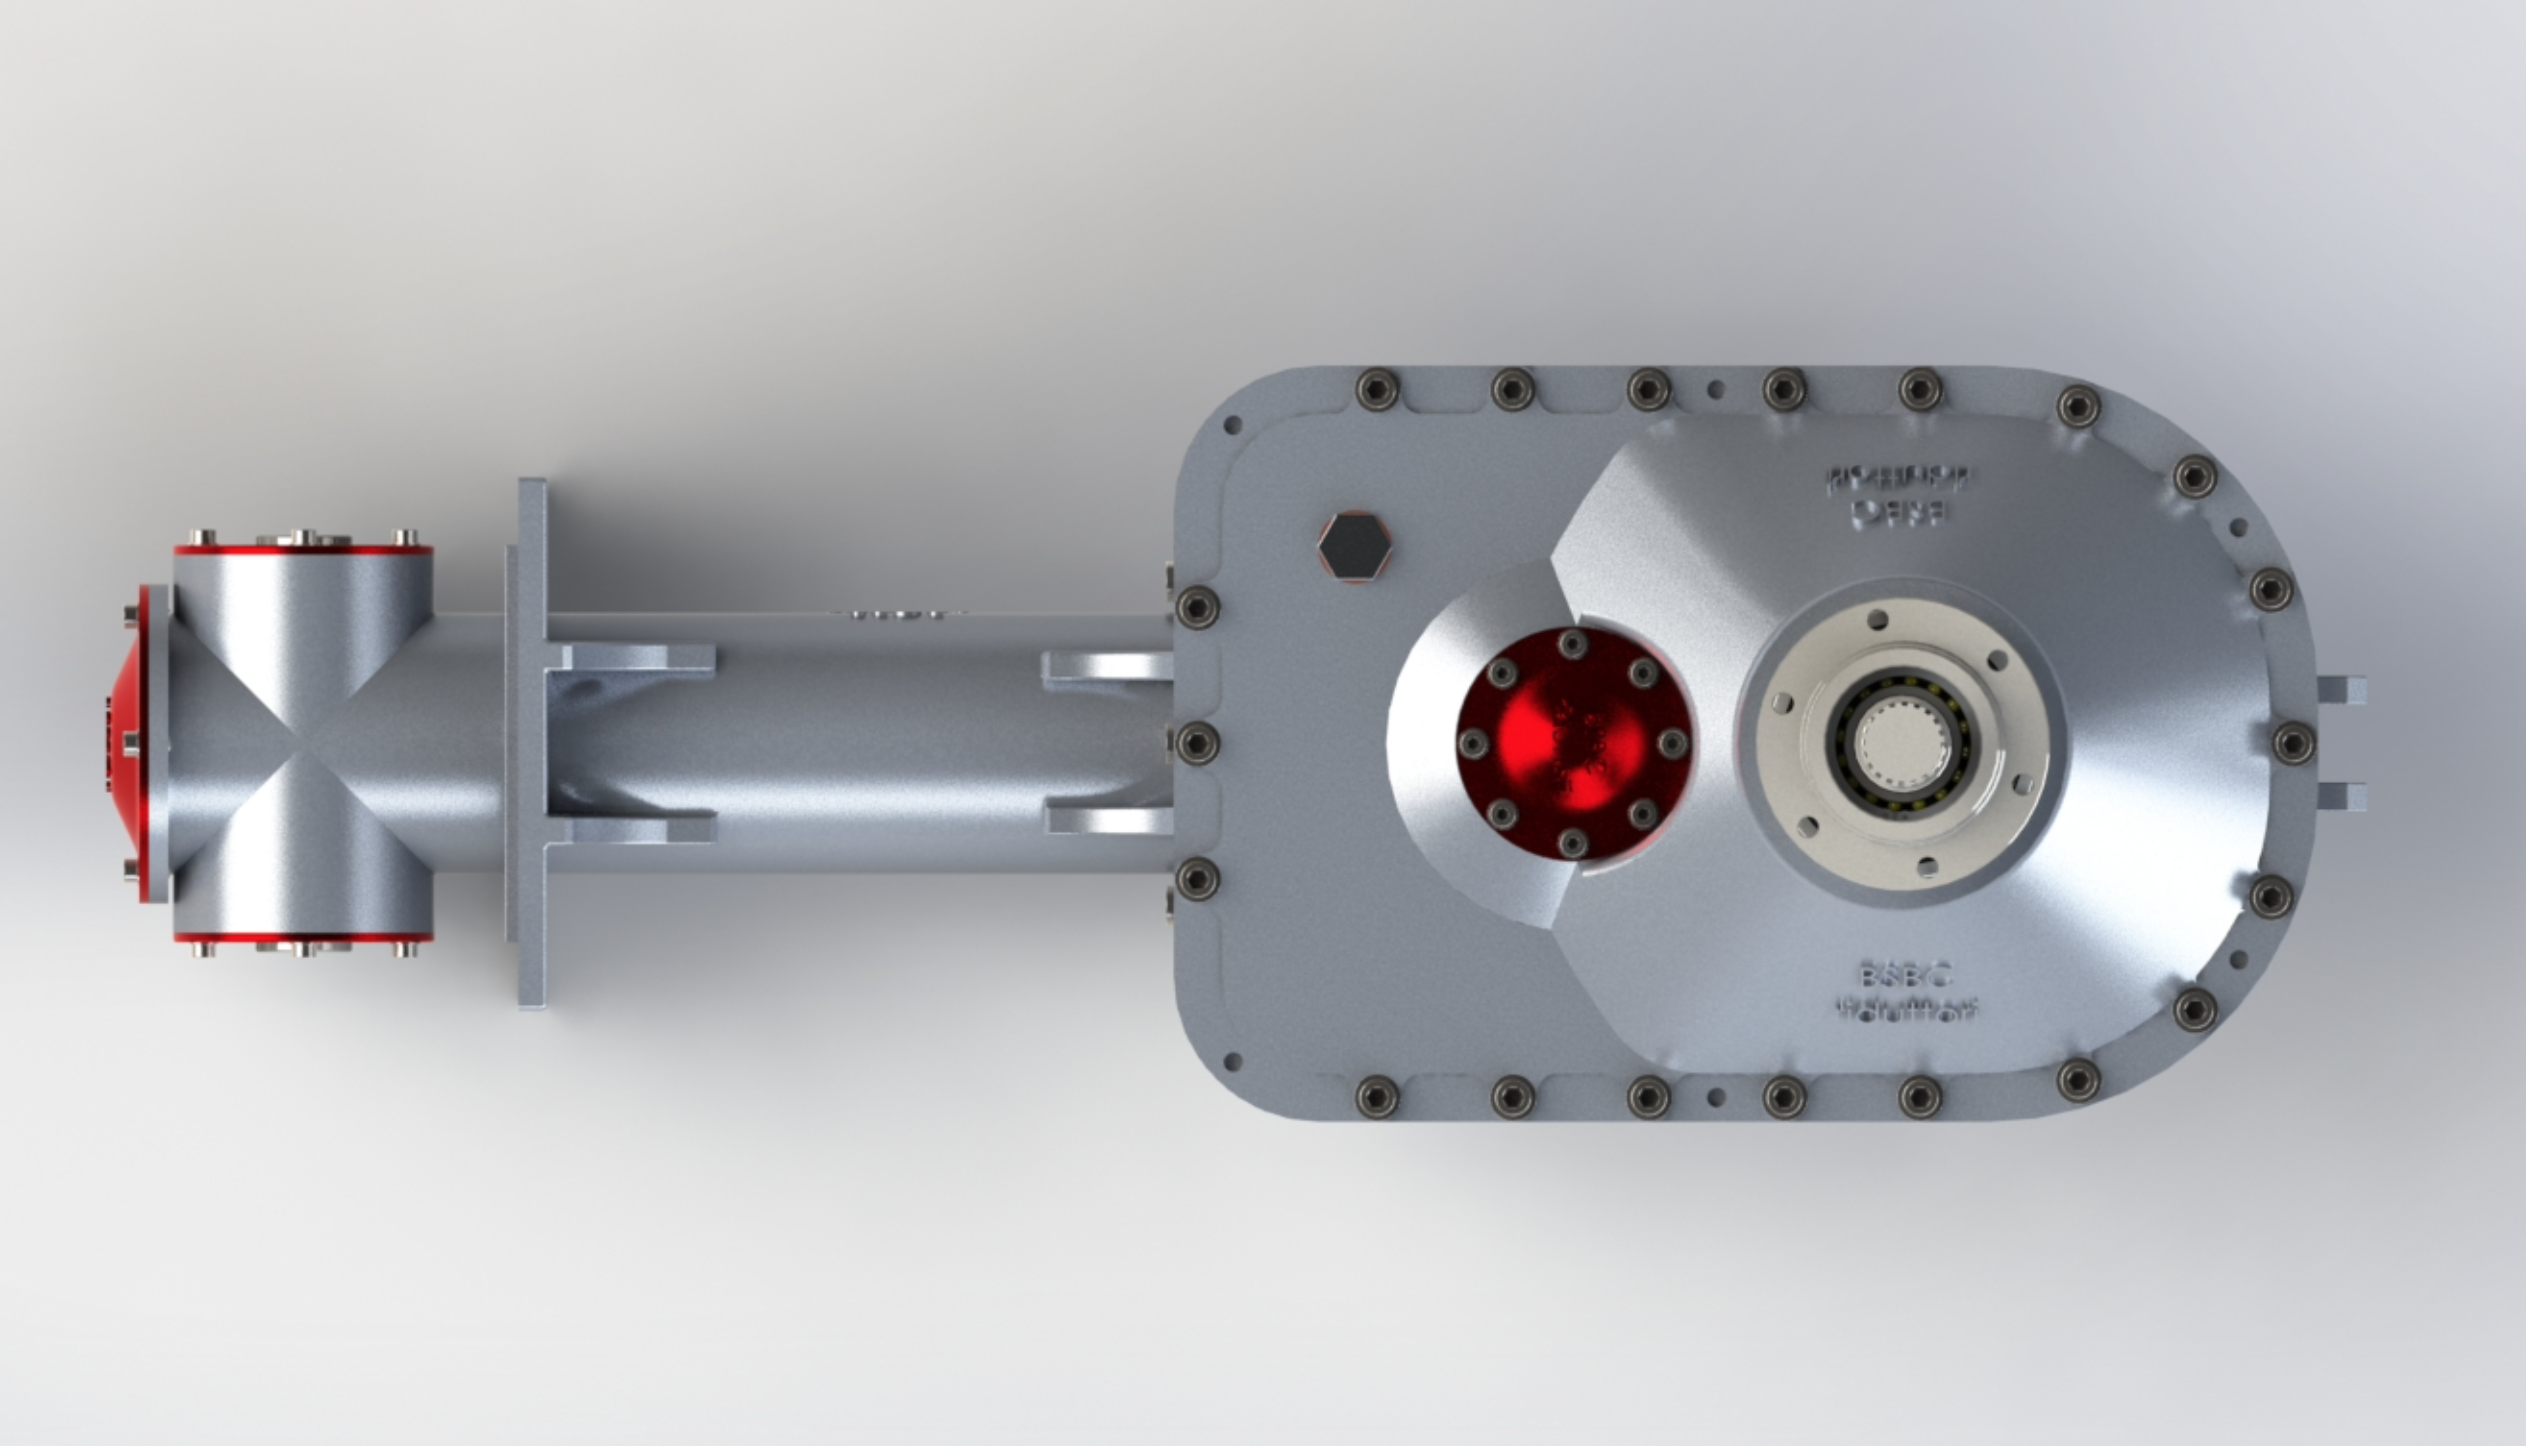
\includegraphics[scale=0.3]{Immagini/RenderingRiduttore4.png}
    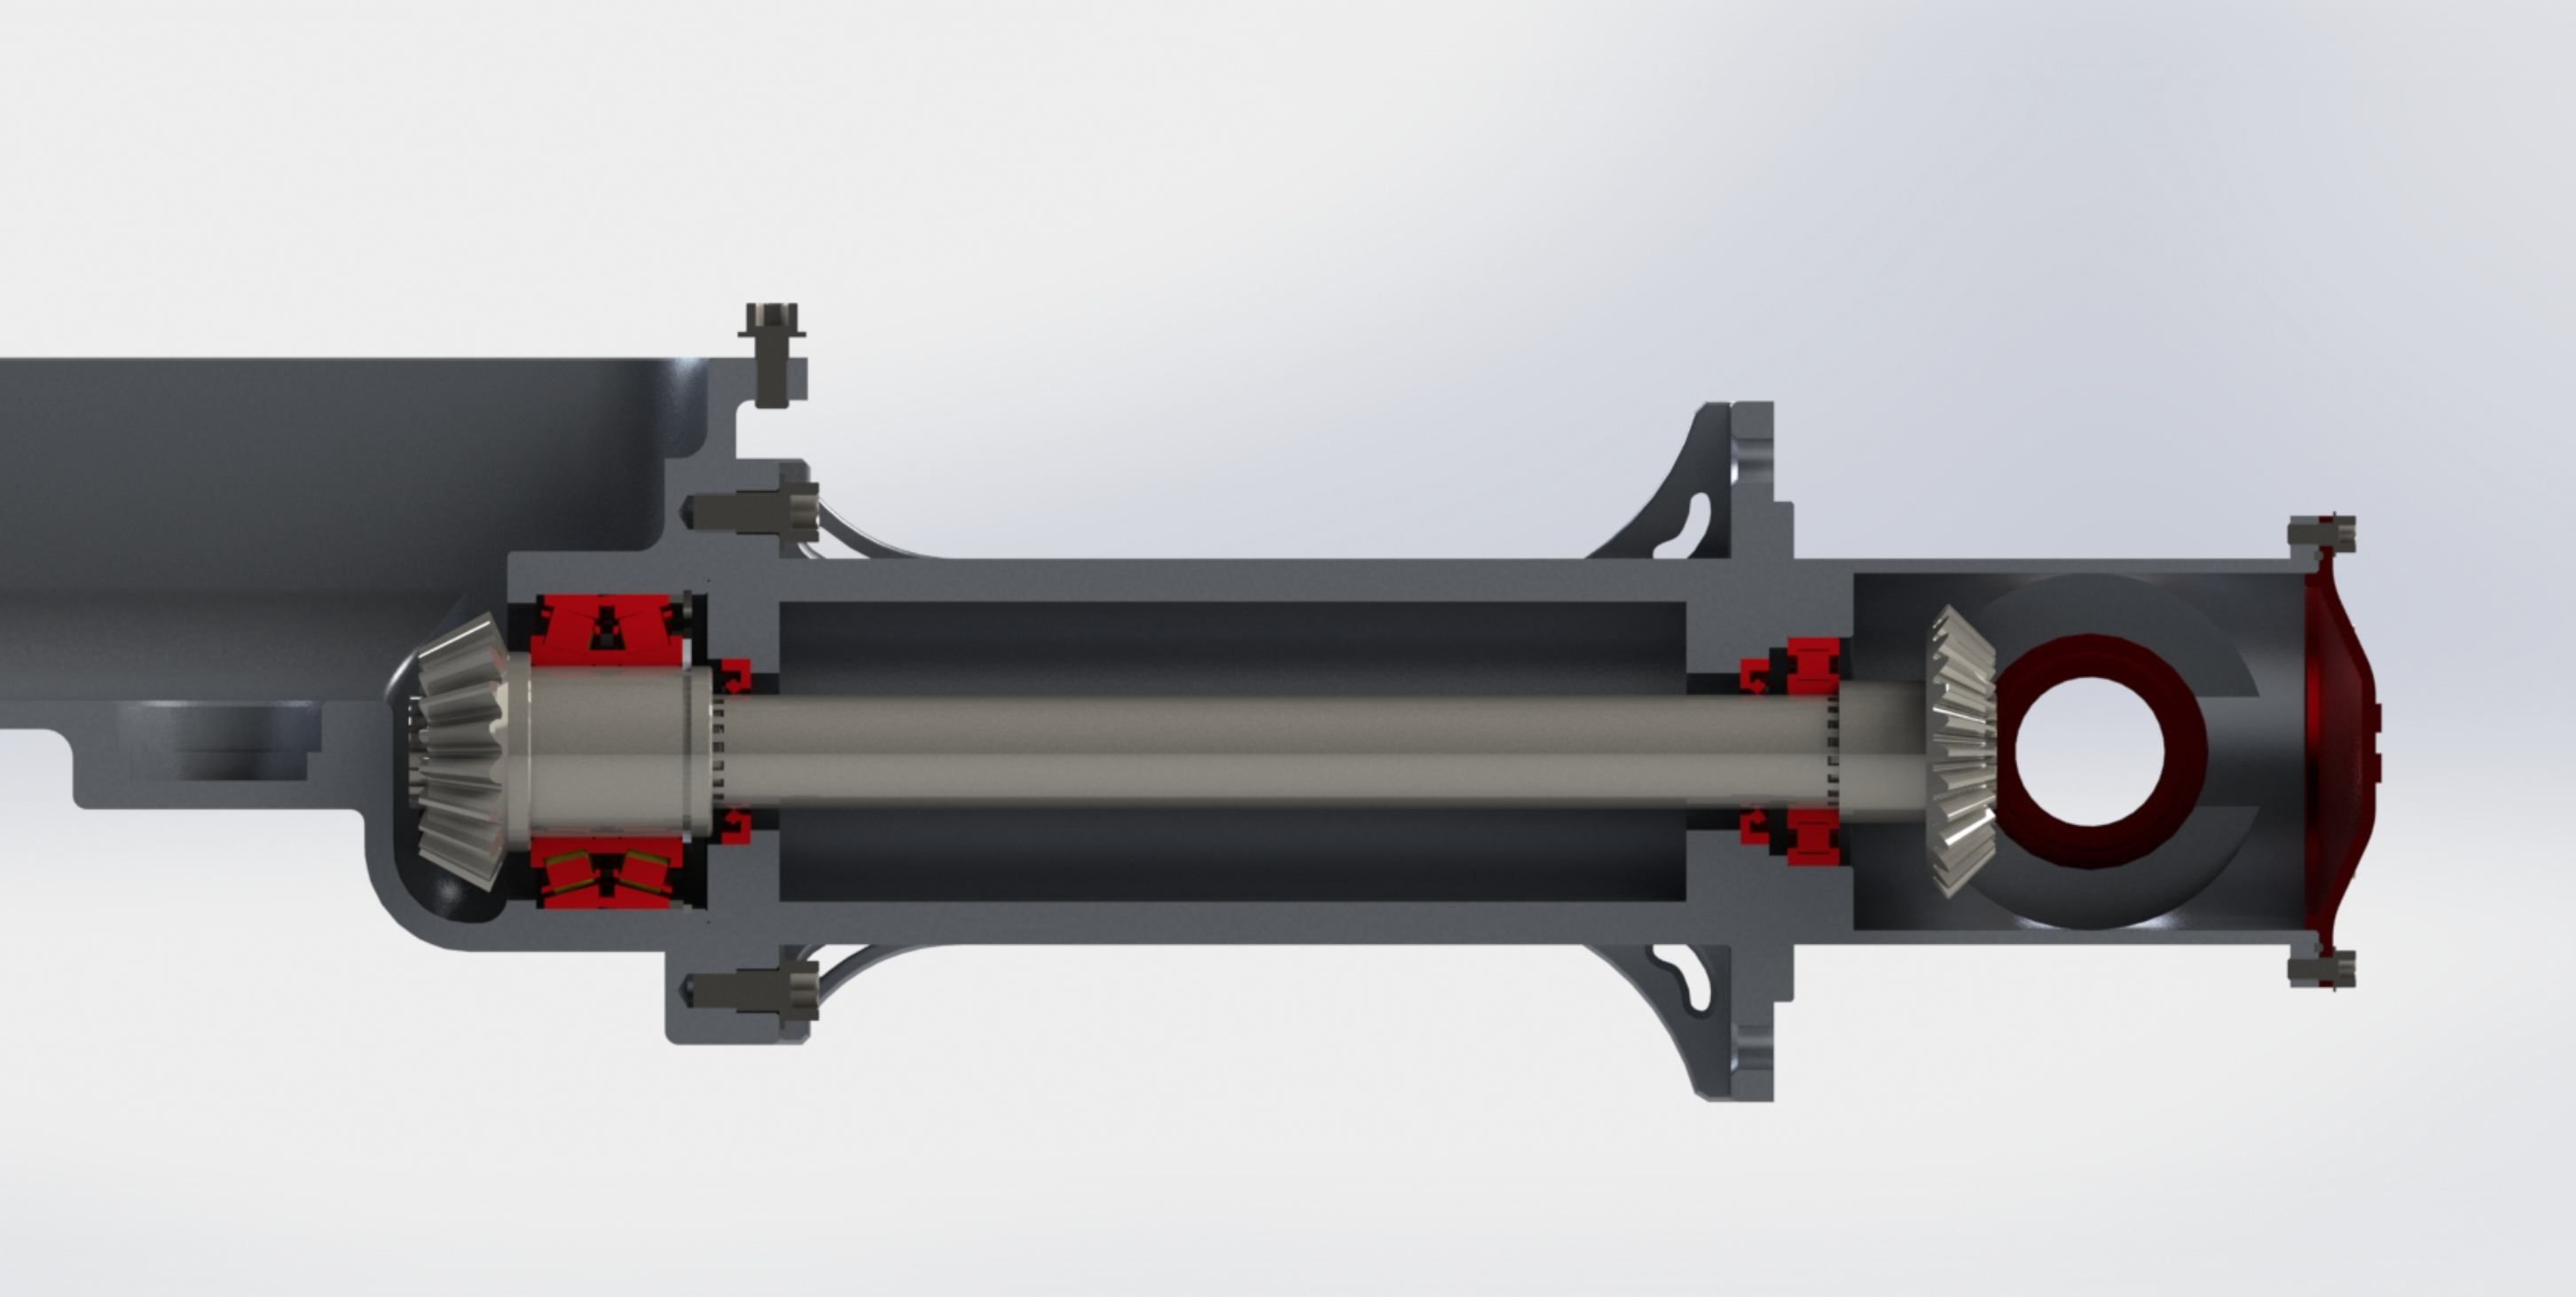
\includegraphics[scale=0.26]{Immagini/RenderingRiduttore5.png}
    \caption{Rendering riduttore modellato tramite software SOLIDWORKS}
    \label{fig:riduttore34}
\end{figure}
\newpage
\begin{figure}[h]
    \centering
    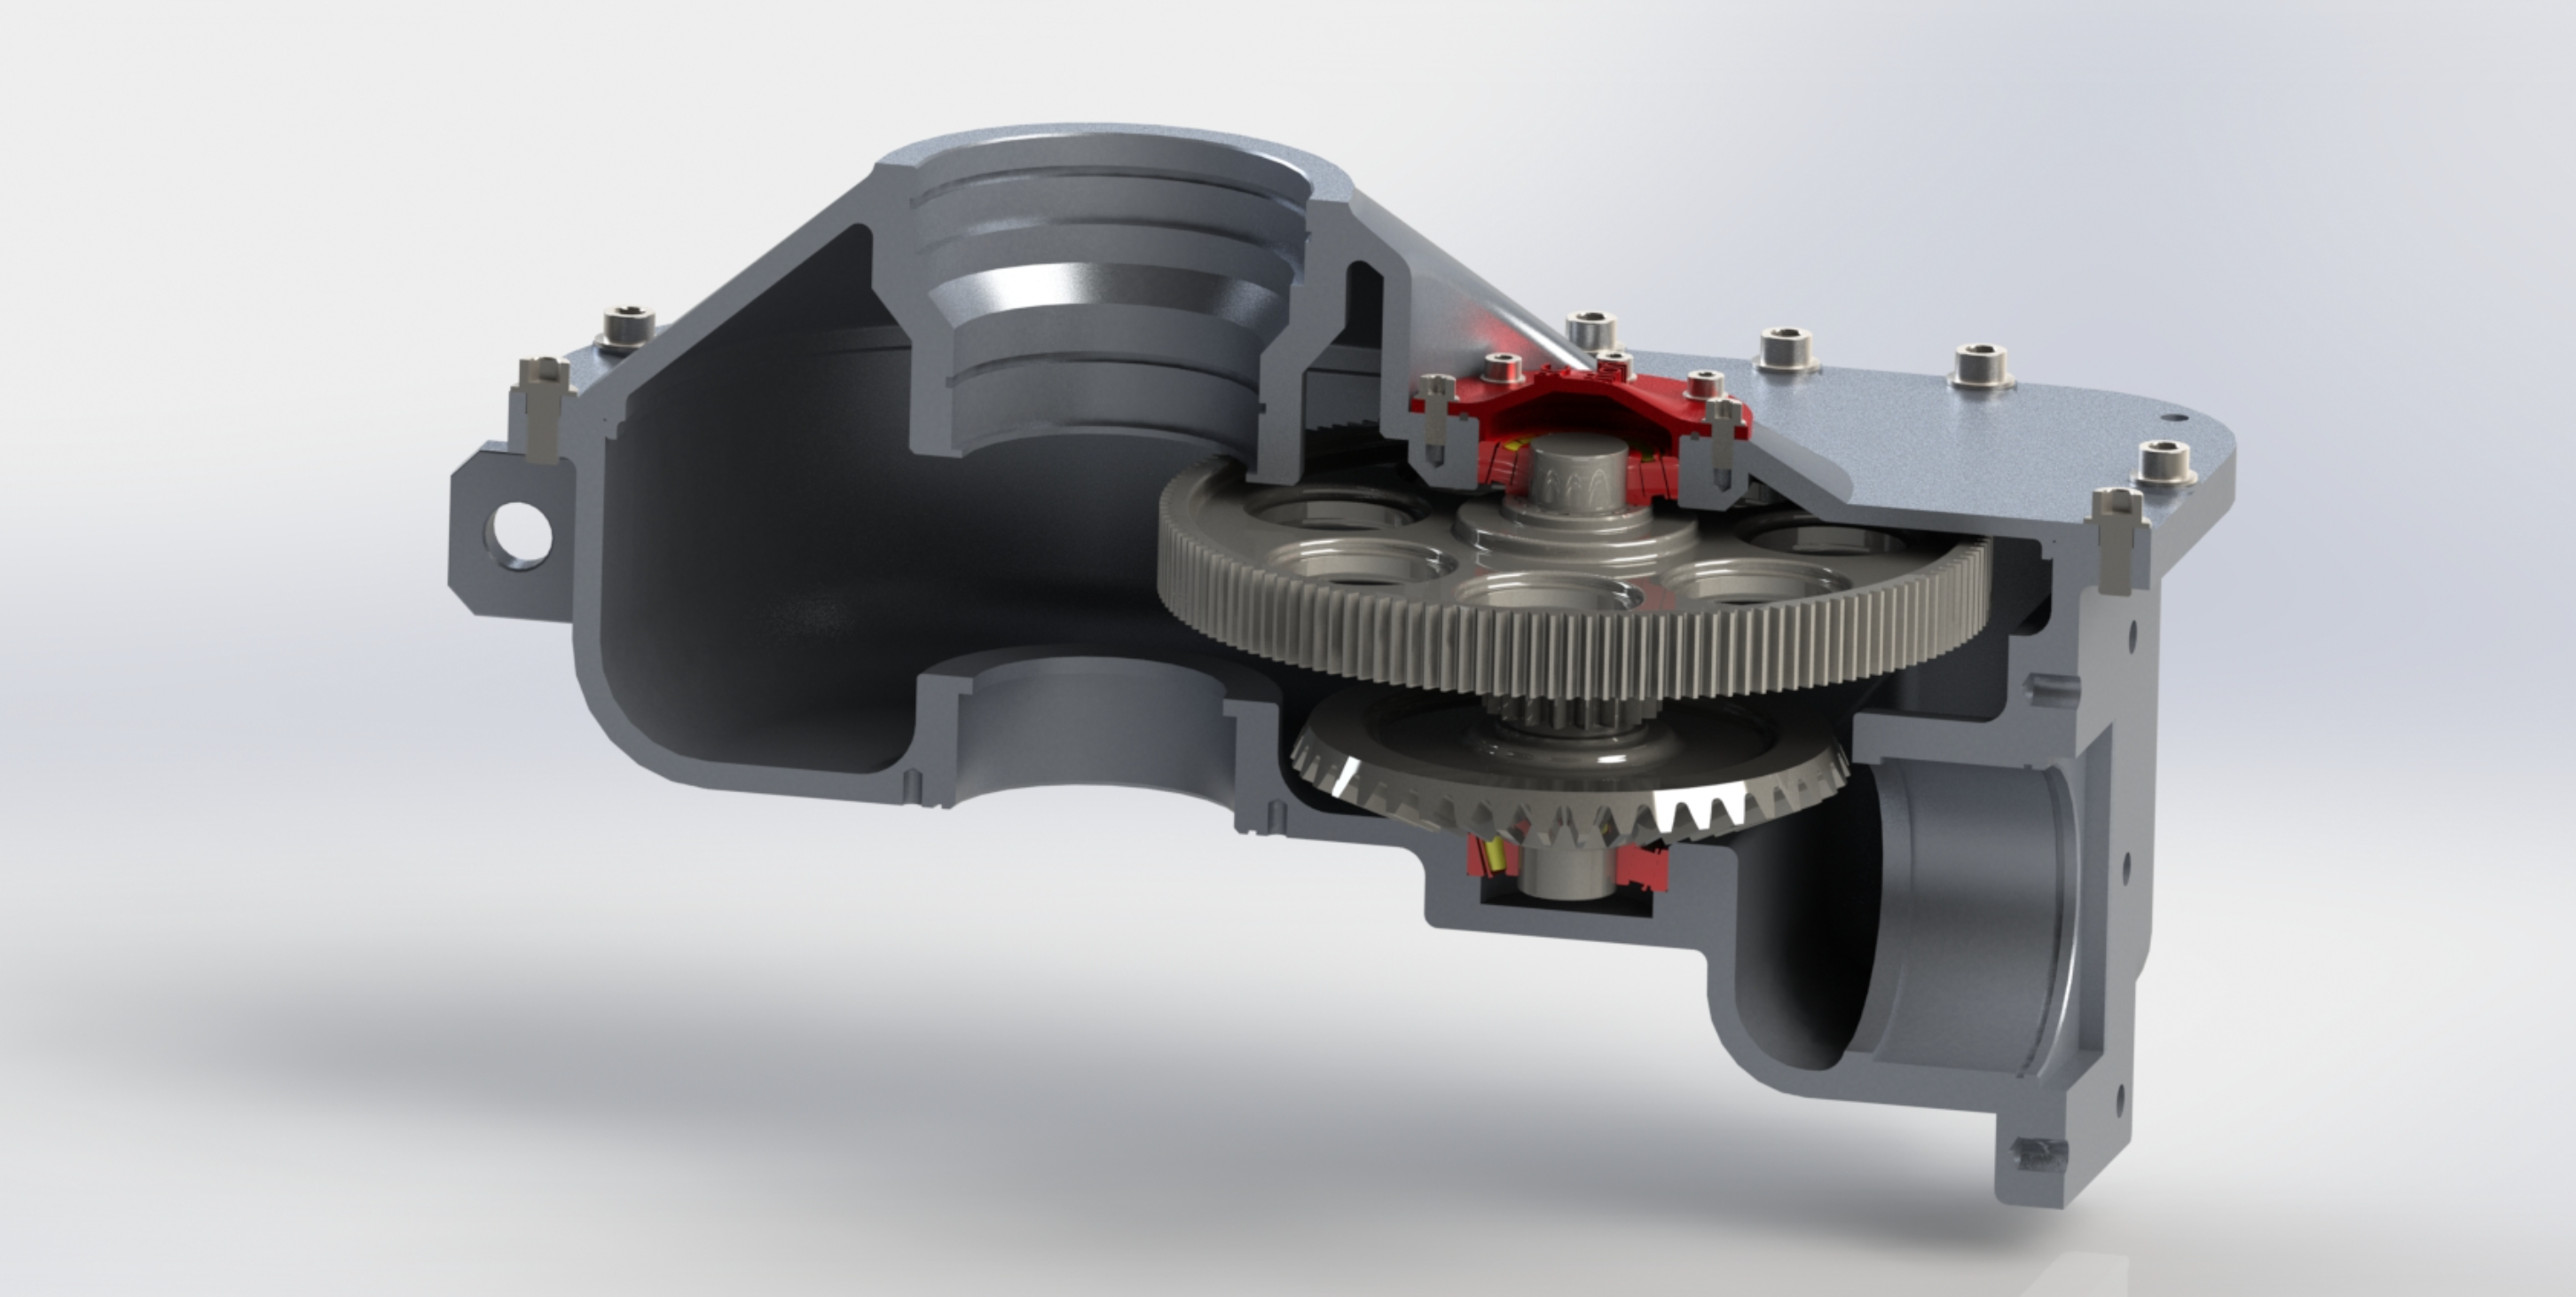
\includegraphics[scale=0.27]{Immagini/RenderingRiduttore6.png}
    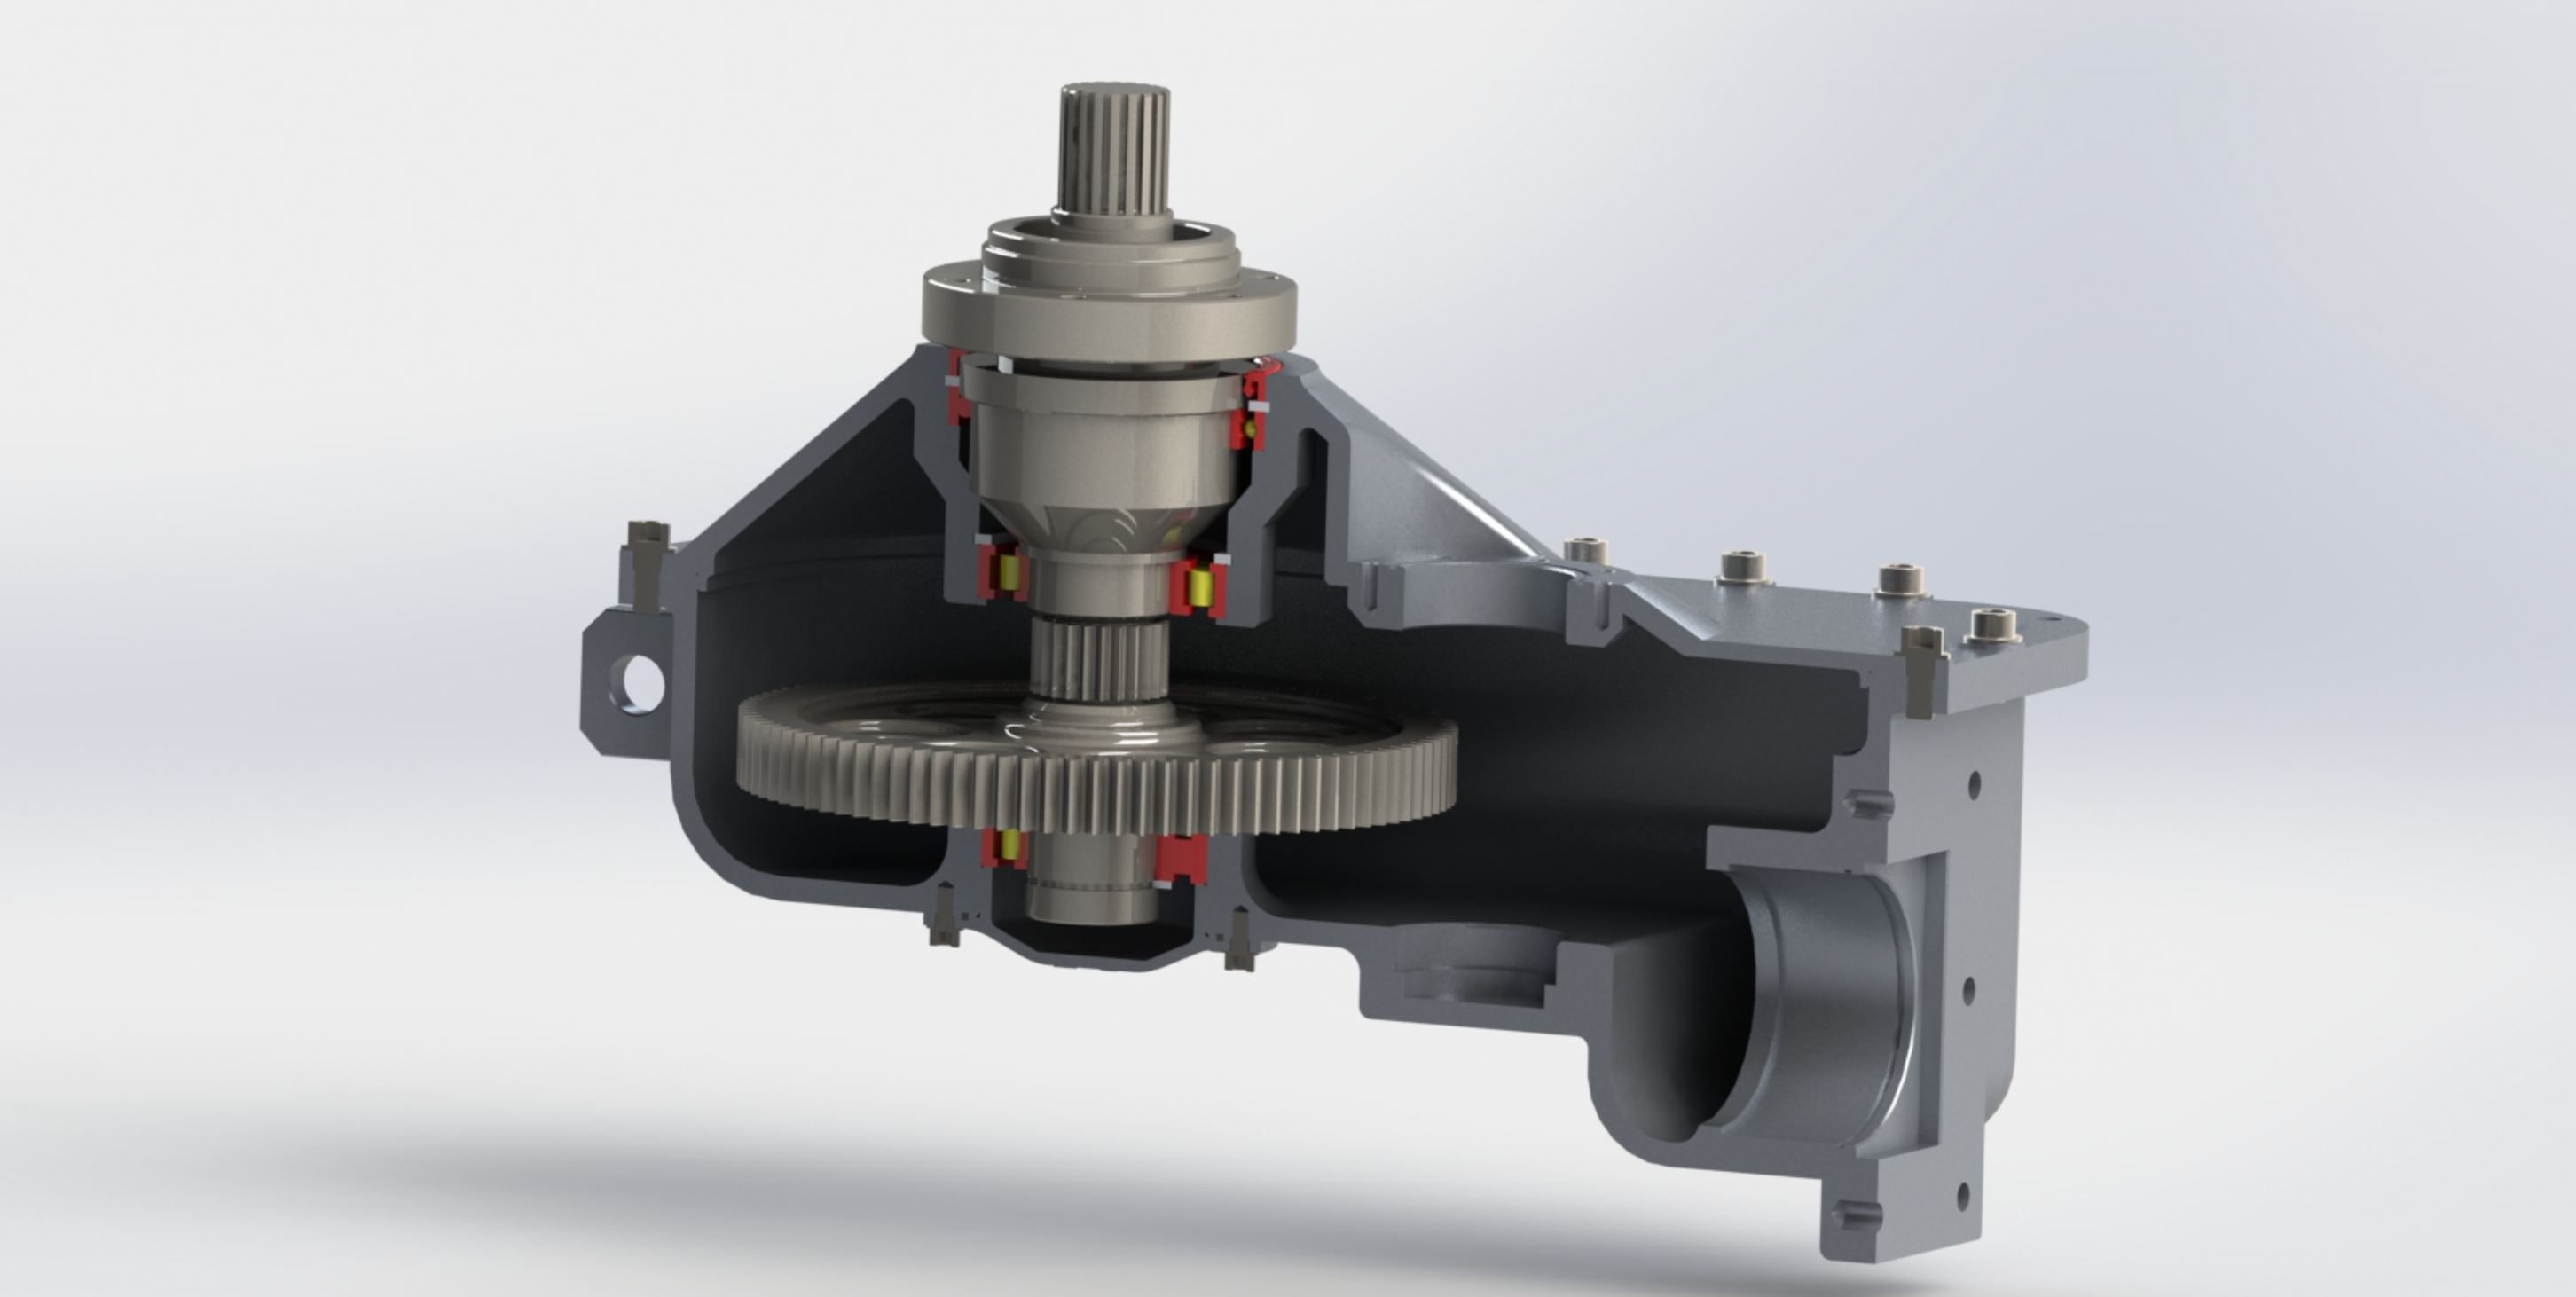
\includegraphics[scale=0.27]{Immagini/RenderingRiduttore7.png}
    \caption{Rendering riduttore modellato tramite software SOLIDWORKS}
    \label{fig:riduttore34}
\end{figure}
\newpage
\begin{figure}[h]
    \centering
     \includegraphics[scale=0.27]{Immagini/RenderingRiduttore8.png}
     \includegraphics[scale=0.27]{Immagini/RenderingRiduttore9.png}
    \caption{Rendering riduttore modellato tramite software SOLIDWORKS}
    \label{fig:my_label}
\end{figure}
